%! suppress = EscapeHashOutsideCommand
%! Author = Theodore Capinski
%! Date = 4/7/2024

% Preamble
\documentclass[11pt]{article}
\let\oldsection\section
\renewcommand\section{\clearpage\oldsection}
\setcounter{section}{-1}
\counterwithin{figure}{section}

% Packages
\usepackage{amsmath}
\usepackage{hyperref}
\usepackage{graphicx}
\usepackage{tikz}
\usepackage{indentfirst}
\usepackage{circuitikz}
\usepackage{calc}
\usepackage{float}

%%%%%%%%%%%%%%%%%%%%%%%%%%%%%%%%%%%%%%%%%%%%%%%%%%%%%%%%%%%%%%%%%%%%%%
% LaTeX Overlay Generator - Annotated Figures v0.0.1
% Created with http://ff.cx/latex-overlay-generator/
%%%%%%%%%%%%%%%%%%%%%%%%%%%%%%%%%%%%%%%%%%%%%%%%%%%%%%%%%%%%%%%%%%%%%%
%\annotatedFigureBoxCustom{bottom-left}{top-right}{label}{label-position}{box-color}{label-color}{border-color}{text-color}
\newcommand*\annotatedFigureBoxCustom[8]{\draw[#5,thick,rounded corners] (#1) rectangle (#2);\node at (#4) [fill=#6,thick,shape=circle,draw=#7,inner sep=2pt,font=\sffamily,text=#8] {\textbf{#3}};}
%\annotatedFigureBox{bottom-left}{top-right}{label}{label-position}
\newcommand*\annotatedFigureBox[4]{\annotatedFigureBoxCustom{#1}{#2}{#3}{#4}{white}{white}{black}{black}}
\newcommand*\annotatedFigureText[4]{\node[draw=none, anchor=south west, text=#2, inner sep=0, text width=#3\linewidth,font=\sffamily] at (#1){#4};}
\newenvironment {annotatedFigure}[1]{\centering\begin{tikzpicture}
                                                   \node[anchor=south west,inner sep=0] (image) at (0,0) { #1};\begin{scope}[x={(image.south east)},y={(image.north west)}]}{\end{scope}\end{tikzpicture}}
%%%%%%%%%%%%%%%%%%%%%%%%%%%%%%%%%%%%%%%%%%%%%%%%%%%%%%%%%%%%%%%%%%%%%%

\newcommand{\todo}[1]{\textcolor{red}{TODO: #1}\PackageWarning{TODO:}{#1!}}

\title{Physics 5BL Lab Report Standing Waves}
\author{T.~Capinski \and A.~Patel}

% Document
\begin{document}
    \maketitle
    \tableofcontents

    \section*{Introduction}\label{sec:introduction}
    \addcontentsline{toc}{section}{Introduction}
    In this lab, we studied the behavior of standing waves on a string. We performed 3 experiments where we held 2 of the following variables constant and varied the other: frequency, tension, and length. We drove the standing wave with a sin wave with an output impedance of 50 $\Omega$ and an amplitude of 10 volts peak to peak.

    In experiment 1, we held the tension constant at a 150-gram hanging mass, equal to 1.47 N of force. We also kept the length constant at 1 meter, while varying the frequency. We found the relationship between each harmonic and the frequency to be linear, with the fit having a chi-squared value of 0.36, an acceptable value. We also found the linear mass density ($\mu$) theoretically and experimentally, calculating 0.0045 + −0.0014 kg/m and 0.0043 + −0.0017 kg/m respectively, which agreed with each other.

    In experiment 2, we held the frequency at 30 Hz and the length at 1.11 meters, varying the hanging mass, thus affecting the tension. todo results

    Lastly, experiment 3 involved varying the length while keeping the frequency at 50 Hz and the hanging mass at 150 grams. We found the relationship between each harmonic and the length to be linear, with the fit having a chi-squared value of 0.22, an acceptable value. We also found the linear mass density ($\mu$) theoretically and experimentally, calculating 0.0045 + −0.0014 kg/m and 0.0040 + −0.0017 kg/m  respectively, which agreed with each other.

    
    \section*{Theory}\label{sec:theory}
    \addcontentsline{toc}{section}{Theory}

    \section{Part 1: Fixed Length and Tension, Varying Frequency}\label{sec:part_1}
    \subsection{Methods}\label{subsec:part_1_methods}
    In part 1, we fixed the length and tension (the hanging mass) of the string but varied the frequency to find the harmonics. We hung a 150-gram mass over a pulley from our string. We had a 292 cm string, but only 1 meter was oscillating, another 72 cm was hanging off the table, and the rest was unused. The total mass of the string was 13 grams. Our setup can be seen in the following picture:

    {todo picture of part 1 setup}

    We varied the frequency to find harmonics 1-7. We measured the frequency, amplitude, and half-frequency, which is the frequency at which the harmonic is the same but the amplitude is half the maximum. We measured the following data:

    \begin{table}[h]
    \centering
    \begin{tabular}{|c|c|c|c|}
    \hline
    \textbf{Harmonic} & \textbf{Freq (Hz)} & \textbf{Amp (cm)} & \textbf{Freq (1/2 A)} \\
    \hline
    1 & 9.14 & 4 & 8.82 \\
    2 & 18 & 3 & 17.6 \\
    3 & 27.41 & 1.3 & 27.9 \\
    4 & 36.89 & 1.1 & 35.9 \\
    5 & 46.30 & 1.1 & 45.4 \\
    6 & 55.50 & 1 & 54.9 \\
    7 & 65.52 & 0.7 & 64.2 \\
    \hline
    \end{tabular}
    \caption{Harmonic frequencies, amplitudes, and half frequencies}
    \label{tab:harmonics}
    \end{table}
    
    
    \subsection{Analysis}\label{subsec:part_1_analysis}
    We created a graph of our data, plotting frequency vs harmonic number. We performed a fit using equation (todo fit equation, number 5 in lab). We then plotted the residuals and found the reduced chi-squared value. This gave us the following graphs:

    (todo insert both part 1 graphs. Caption: frequency vs harmonic graph and residuals for part 1.)

    From these graphs, we can see a linear fit is a good fit for our data, as the line hits all our data points and our residuals are randomly scattered around the 0 line. We can then calculate the linear mass density ($\mu$) of the string using equation (todo equation for LMD, in lab notebook)
    
    where:
    \begin{align*}
    \text{length} &= 1 \, \text{m} \\
    g &= 9.8 \, \text{m/s}^2 \\
    \text{tension} &= hanging mass \cdot g\\
    \end{align*}
    
    $\mu$ calculated from the slope is denoted as $\mu_{\text{exp}}$, which is calculated as:
    
    \begin{equation}
    \mu_{\text{exp}} = 0.0043 +- 0.0017 kg/m
    \end{equation}
    
    The theoretical value of $\mu$, denoted as $\mu_{\text{th}}$, is calculated using:
    
    \begin{equation}
    \mu_{\text{th}} = \frac{0.013}{2.92} = 0.0045 +- 0.0014 kg/m
    \end{equation}

    We can then do an agreement test between the values, using equation (todo agreement equation).

    \begin{align*}
    |0.0045 - 0.0043| &< 2 \sqrt{(0.0017)^2 + (0.0014)^2} \\
    0.0002 &< 2 \sqrt{0.00002889 + 0.0000196} \\
    0.0002 &< 2 \sqrt{0.00004849} \\
    0.0002 &< 2 \times 0.00696 \\
    0.0002 &< 0.01392
    \end{align*}

    From this, we can see that our value for linear mass density agrees with the theoretical value. We can also observe that our chi-squared value was 0.36. This is an acceptable value. This indicates that the experimental data obtained align well with the theoretical model. This suggests that the measurements were carried out accurately and the uncertainties were estimated reliably. The results can be considered trustworthy and can support conclusions drawn from the experiment regarding the behavior of the harmonic oscillating string. 


    
    \subsection{Conclusion}\label{subsec:part_1_conclusion}
    This experiment investigated the relationship between the resonant frequency of a vibrating string and the harmonic number. We were able to accurately measure the resonant frequencies for the first 7 harmonics while ensuring proper node placement at both ends of the string. The uncertainties associated with our measurements were then found from the half amplitude of the oscillations. Plotting the measured resonant frequencies against the harmonic number and performing a weighted least squares fit using equation (todo fit equation) showed the fit was appropriate for our data. We then measured the linear mass density both theoretically and experimentally, which agreed with each other based on our agreement test. Lastly, we found that our chi-squared value was accurate, further showing the goodness of the fit.

    
    \section{Part 2: Fixed Length and Frequency, Varying Tension }\label{sec:part_2}


    \subsection{Methods}\label{subsec:part_2_methods}

    For the second part of this lab, we fixed the length and frequency of the oscillating string, while varying the tension.
    We made the frequency 30 hz and kept the length at 1.11 meters.
    Our setup can be seen in the following picture:

    \begin{figure}[H]
    \centering
        \begin{annotatedFigure}
        {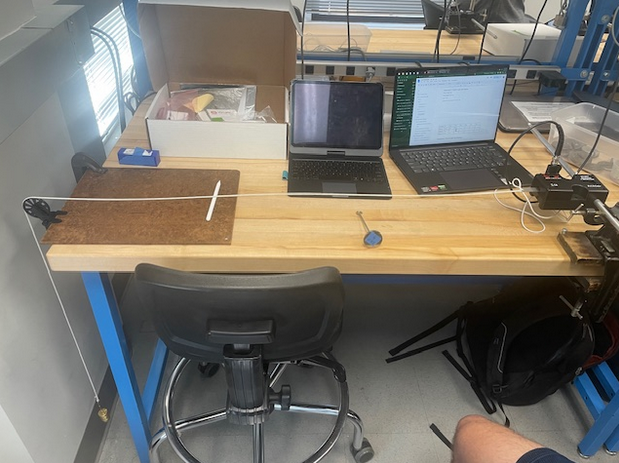
\includegraphics[width=1.0\linewidth]{resources/images/2 setup}}
            \annotatedFigureBox{0.3011,0.5159}{0.729,0.6338}{A}{0.3011,0.5159}%bl
            \annotatedFigureBox{0.821,0.5348}{0.982,0.6654}{B}{0.821,0.5348}%bl
            \annotatedFigureBox{0.0268,0.3482}{0.0994,0.5922}{C}{0.0268,0.3482}%bl
        \end{annotatedFigure}
    \caption{Part 2 setup, showing (a) as the string, (b) as the string oscillator, and (c) as the pulley and hanging mass (off-screen).}
    \label{fig:part_2_setup}
    \end{figure}

    We varied the tension to find harmonics 2--7.
    This was achieved by changing the hanging mass.
    When the tension was increased, the harmonics increased.
    As we found the desired harmonic, we measured the tension, amplitude, and half-tension (which refers to the tension at which the harmonic is the same but the amplitude is half the maximum).
    The half-measurement was used to form an uncertainty range for the tension.
    We repeated this process for each harmonic.

    To avoid tediously changing the tension, we estimated how much tension should be applied to the string to achieve the desired harmonic.
    We then adjusted the tension until the desired harmonic was observed.
    The equation
    \begin{align*}
        n = 2fL \sqrt{\frac{\mu}{T}}
    \end{align*}
    relates the harmonic, n, to the tension, T\@.
    In this equation, $\mu$ is the linear mass density of the string.
    However, because the string stretches, $\mu$ is not constant.
    Instead, it changes with tension.

    The adjusted linear mass density is given by
    \begin{align*}
        \mu_{stretched} = \frac{\mu_0}{(mk+10)/10}
    \end{align*}
    where $mu_0$ is the linear mass density of the string at rest, m is the hanging mass, and k is the spring constant of the string.
    The spring constant was estimated by measuring the length of a 10cm section of the string as we increased tension.

    With this information, we can calculate the theoretical tension for each harmonic, shown in Figure\ref{fig:theoretical_tension}.

    \begin{figure}[H]
        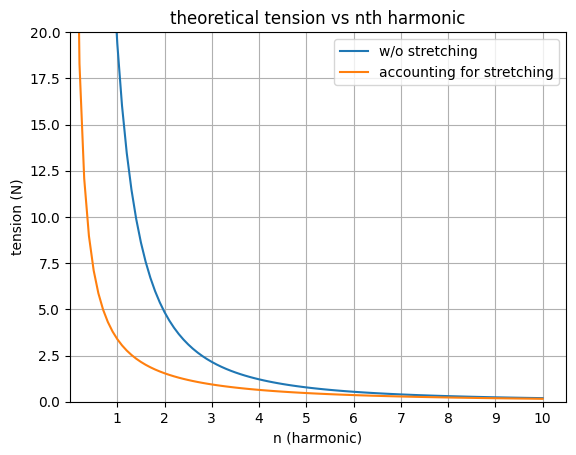
\includegraphics[width=0.5\textwidth]{/resources/images/2 theoretical tension graph}
        \caption{Theoretical tension vs. harmonic graph}
        \label{fig:theoretical_tension}
    \end{figure}

    We used this graph to more easily find the desired harmonic.

    \subsection{Analysis}\label{subsec:part_2_analysis}

    Our measured data was as follows:
    \begin{table}[H]
        \centering
        \begin{tabular}{|c|c|c|c|}
        \hline
        \textbf{Harmonic} & \textbf{Mass (g)} & \textbf{Half Mass (g)} \\
        \hline
        2 & 340 & 355   \\
        3 & 200 & 210   \\
        4 & 120 & 125   \\
        5 & 80 & 75     \\
        6 & 55 & 50     \\
        7 & 40 & 35     \\
        \hline
        \end{tabular}
        \caption{Harmonic tension, amplitudes, and half tensions. The tension is the mass \$times$ gravity.}
        \label{tab:harmonic_tensions}
    \end{table}

    We created a graph of our data, plotting tension vs harmonic number.
    We performed a fit using equation (todo fit equation, number 5 in lab).
    This fit found both the initial linear mass density and the spring constant.
    We then plotted the residuals and conducted an agreement test between the theoretical and experimental values of the linear mass density.
    This gave us the following graphs:

    \begin{figure}[H]
        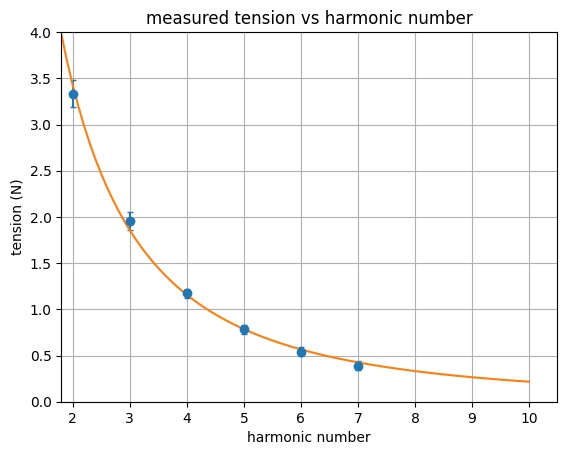
\includegraphics[width=0.5\textwidth]{/resources/images/2 measured tension graph}
        \caption{Tension vs. harmonic graph}
        \label{fig:measured_tension}
    \end{figure}

    \begin{figure}[H]
        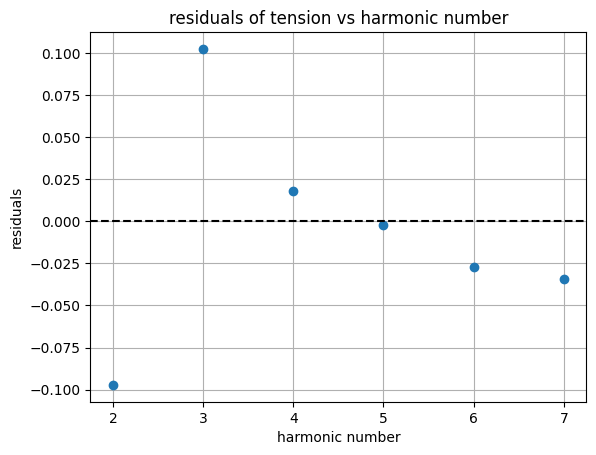
\includegraphics[width=0.5\textwidth]{/resources/images/2 measured tension residuals}
        \caption{Residuals for tension vs. harmonic graph}
        \label{fig:measured_tension_residuals}
    \end{figure}

    From these graphs, we can see a linear fit is a good fit for our data, as the line hits all our data points and our residuals are randomly scattered around the 0 line.
    The agreement test between the theoretical and experimental values of the linear mass density says
    \begin{align*}
        |0.0045 - 0.0043| &< 2 \sqrt{(0.0017)^2 + (0.0014)^2} \\
        0.0002 &< 2 \sqrt{0.00002889 + 0.0000196} \\
        0.0002 &< 2 \sqrt{0.00004849} \\
        0.0002 &< 2 \times 0.00696 \\
        0.0002 &< 0.01392
    \end{align*}
    that means our value for linear mass density agrees with the theoretical value.

    From the fit, we can also observe that the spring constant was higher than initially estimated.
    This is likely due to the string stretching more than we anticipated, or due to a faulty initial estimate.
    Regardless, the fit was still good, and the agreement test passed.

    \subsection{Conclusion}\label{subsec:part_2_conclusion}

    \todo{conclusion}

    \section{Part 3: Fixed Tension and Frequency, Varying Length}\label{sec:part_3}
    \subsection{Methods}\label{subsec:part_3_methods}
    For the last part of this lab, we fixed the tension (hanging mass) and frequency of the oscillating string, while varying the length of it. We made the hanging mass 150 grams and kept the frequency at 50 hz. Our setup can be seen in the following picture:

    TODO part 3 setup (probably same as others)

    We varied the length to find harmonics 1-7. We measured the length, amplitude, and length, which is the length at which the harmonic is the same but the amplitude is half the maximum. We measured the following data:

    \begin{table}[h]
    \centering
    \begin{tabular}{|c|c|c|c|}
    \hline
    \textbf{Harmonic} & \textbf{Length (cm)} & \textbf{Amplitude (cm)} & \textbf{Half Length (cm)} \\
    \hline
    1 & 20 & 2 & 18 \\
    2 & 39 & 1.7 & 36 \\
    3 & 57.5 & 1.6 & 55 \\
    4 & 76 & 1.4 & 74 \\
    5 & 95 & 1.3 & 94 \\
    6 & 113.5 & 1.1 & 113 \\
    7 & 133 & 1.1 & 132.5 \\
    \hline
    \end{tabular}
    \caption{Harmonic lengths, amplitudes, and half lengths}
    \label{tab:harmonic_lengths}
    \end{table}
    
    \subsection{Analysis}\label{subsec:part_3_analysis}
    We created a graph of our data, plotting LENGTH vs harmonic number. We performed a fit using equation (todo fit equation, number 5 in lab). We then plotted the residuals and found the reduced chi-squared value. This gave us the following graphs:

    (todo insert both part 3 graphs. Caption: LENGTH vs harmonic graph and residuals for part 3.)

    From these graphs, we can see a linear fit is a good fit for our data, as the line hits all our data points and our residuals are randomly scattered around the 0 line. We can then calculate the linear mass density ($\mu$) of the string using equation (todo equation for LMD, in lab notebook)
    
    where:
    \begin{align*}
    \text{frequency} &= 50 \, \text{Hz} \\
    g &= 9.8 \, \text{m/s}^2 \\
    \text{tension} &= 0.150 \cdot g\\
    \end{align*}
    
    $\mu$ calculated from the slope is denoted as $\mu_{\text{exp}}$, which is calculated as:
    
    \begin{equation}
    \mu_{\text{exp}} = 0.0040 +- 0.0017 kg/m
    \end{equation}
    
    The theoretical value of $\mu$, denoted as $\mu_{\text{th}}$, is calculated using:
    
    \begin{equation}
    \mu_{\text{th}} = \frac{0.013}{2.92} = 0.0045 +- 0.0014 kg/m
    \end{equation}

    We can then do an agreement test between the values, using equation (todo agreement equation).

    \begin{align*}
    |0.0045 - 0.0040| &< 2 \sqrt{(0.0014)^2 + (0.0017)^2} \\
    0.0005 &< 2 \sqrt{0.0014^2 + 0.0017^2} \\
    0.0005 &< 2 \sqrt{0.0000196 + 0.0000289} \\
    0.0005 &< 2 \sqrt{0.0000485} \\
    0.0005 &< 2 \times 0.00696 \\
    0.0005 &< 0.01392
    \end{align*}

    From this, we can see that our value for linear mass density agrees with the theoretical value. We can also observe that our chi-squared value was 0.22. This is an acceptable value. This indicates that the experimental data obtained align well with the theoretical model. This suggests that the measurements were carried out accurately and the uncertainties were estimated reliably. The results can be considered trustworthy and can support conclusions drawn from the experiment regarding the behavior of the harmonic oscillating string. 

    
    \subsection{Conclusion}\label{subsec:part_3_conclusion}
    This experiment investigated the relationship between the length of a vibrating string and the harmonic number. We were able to accurately measure the lengths for the first 7 harmonics while ensuring proper node placement at both ends of the string. The uncertainties associated with our measurements were then found from the half amplitude of the oscillations. Plotting the measured lengths against the harmonic number and performing a weighted least squares fit using equation (todo fit equation) showed the fit was appropriate for our data. We then measured the linear mass density both theoretically and experimentally, which agreed with each other based on our agreement test. Lastly, we found that our chi-squared value was accurate, further showing the goodness of the fit.

    \section{Lab Conclusion}\label{sec:lab_conclusion}
    In this lab, we investigated standing waves on a string under fixed tension and explored how the frequency of oscillation relates to the string's length and tension. Using a vibrating source, we observe the formation of harmonics by sweeping through driving frequencies, lengths, and hanging masses and analyzed their relationships. By conducting these experiments, we aimed to determine the mass density of the string and compare it to theoretical values, while also considering potential improvements to the experimental methods for better accuracy and results.
    
    Experiment 1 involved fixing the length and tension (the hanging mass) of the string but varying the frequency to find the harmonics. We found the relationship between each harmonic and the frequency to be linear and calculated the linear mass density of the string theoretically and experimentally, which agreed with each other. We concluded that our data accurately represented the relationship between frequency and the harmonics.

    Experiment 2 involved fixing the length and frequency of the string but varying the tension (the hanging mass) to find the harmonics. todo results

    Experiment 3 involved fixing the tension and frequency of the string but varying the length to find the harmonics. We found the relationship between each harmonic and the length to be linear and calculated the linear mass density of the string theoretically and experimentally, which agreed with each other. We concluded that our data accurately represented the relationship between frequency and the harmonics.

    Overall, through our exploration of standing waves on a string under varying conditions of tension and length, we gained insights into the fundamental principles governing wave behavior and the relationship between frequency, wavelength, and harmonic formation. This hands-on experimentation provided a practical understanding of wave phenomena and reinforced theoretical concepts, paving the way for further investigations into complex wave systems.
    
    \appendix
    \section{References}\label{sec:references}

    Lab Manual


\end{document}